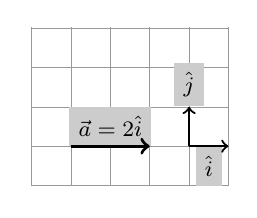
\begin{tikzpicture}[scale=0.5, help lines/.style={black!40,very thin}]
	\clip (-1.1,-1.1) rectangle (4.01,3.01);

	% Grid
	\draw[help lines] (-1,-1) grid +(8,9);

	% \vec a
	\draw (1,0) node[anchor=south, fill=black!20!white] {\footnotesize $\vec a = 2\hat i$};
	\draw[very thick] [->] (0,0) -- (2,0);

	% \hat i
	\draw (3.5,0) node[anchor=north, fill=black!20!white] {\footnotesize $\hat i$};
	\draw[thick] [->] (3,0) -- ++(1,0);

	% \hat j
	\draw (3,1) node[anchor=south, fill=black!20!white] {\footnotesize $\hat j$};
	\draw[thick] [->] (3,0) -- ++(0,1);
\end{tikzpicture}
